\documentclass{article}
\usepackage[margin=1in]{geometry}
\usepackage{tabularx}
\usepackage{array}
\usepackage{booktabs}
\usepackage{xcolor}
\usepackage{amsmath}
\usepackage[T1]{fontenc}
\usepackage[spanish,es-nodecimaldot]{babel}
\usepackage{graphicx,enumitem,fancyhdr,listings,hyperref}
\definecolor{azul}{HTML}{1B2A5E}
\definecolor{dorado}{HTML}{E5B300}
\definecolor{fondo}{HTML}{F3F6FA}
\hypersetup{colorlinks=true,urlcolor=azul,pdftitle={Respuestas - Ejercicios Econometría Taller 1},pdfauthor={Iván Canales}}
\pagestyle{fancy}\fancyhf{}
\fancyhead[L]{\small\color{azul}Econometría - Taller 1}
\setlength{\headheight}{32pt}
\fancyhead[R]{
\includegraphics[height=0.95cm]{../Logo_UTFSM.png}}
\fancyfoot[C]{\small\thepage}
\renewcommand{\headrulewidth}{0.4pt}
\setlength{\parindent}{0pt}\setlength{\parskip}{5pt}
\setlist[enumerate]{leftmargin=*,itemsep=13pt,parsep=4pt}
\lstset{language=R,basicstyle=\ttfamily\small,backgroundcolor=\color{fondo},frame=single,rulecolor=\color{fondo},breaklines=true,columns=fullflexible,keepspaces=true,showstringspaces=false,xleftmargin=6pt,xrightmargin=6pt,aboveskip=6pt,belowskip=6pt}
\newcommand{\codigo}[1]{\texttt{\detokenize{#1}}}
\newcommand{\captura}[3]{\begin{minipage}[t]{0.48\linewidth}\centering\includegraphics[width=\linewidth,height=#3,keepaspectratio]{colab-#1.png}\par\vspace{2pt}{\footnotesize\color{azul}\textbf{#1.} #2}\end{minipage}}
\lstset{basicstyle=\ttfamily\footnotesize,literate={á}{{\'a}}1 {é}{{\'e}}1 {í}{{\'i}}1 {ó}{{\'o}}1 {ú}{{\'u}}1 {ñ}{{\~n}}1 {ü}{{\"u}}1}
\newcommand{\respuesta}[1]{{\Large\bfseries\color{azul}#1\par}\vspace{3pt}{\color{dorado}\hrule height 1pt}\vspace{7pt}}
\begin{document}
{\LARGE\bfseries\color{azul}Respuestas - Ejercicios Econometría Taller 1\par}
{\large Introducción a la computación estadística y econometría\par}
\vspace{8pt}
\respuesta{1. Nombre y apellido alternados}
Se utilizan Ana y Perez como ejemplo. Diez iteraciones muestran cinco veces cada texto, de manera alternada. Reemplaza estos valores por tu nombre y tu apellido.

\begin{minipage}[t]{0.48\linewidth}\textbf{Con for}
\begin{lstlisting}
nombre <- "Ana"
apellido <- "Perez"
for (i in 1:10) {
  if (i %% 2 == 1) {
    print(nombre)
  } else {
    print(apellido)
  }
}
\end{lstlisting}
\end{minipage}\hfill\begin{minipage}[t]{0.48\linewidth}\textbf{Con while}
\begin{lstlisting}
i <- 1
while (i <= 10) {
  if (i %% 2 == 1) {
    print(nombre)
  } else {
    print(apellido)
  }
  i <- i + 1
}
\end{lstlisting}
\end{minipage}

El resto de dividir \codigo{i} por 2 se obtiene con \texttt{i \%\% 2}: es 1 en las posiciones impares y 0 en las pares. Por eso se imprime primero el nombre y después el apellido. En el \codigo{while}, aumentar \codigo{i} permite llegar al final.

\vspace{8pt}\respuesta{2. Sucesión hasta -20}
Hay 40 posiciones: cada número de 1 a 20 aparece una vez positivo y una vez negativo. \codigo{ceiling(i / 2)} redondea hacia arriba y genera 1, 1, 2, 2, etc.; la condición elige el signo.

\begin{minipage}[t]{0.48\linewidth}\textbf{Con for}
\begin{lstlisting}
sucesion_for <- numeric(40)
for (i in 1:40) {
  numero <- ceiling(i / 2)
  if (i %% 2 == 1) {
    sucesion_for[i] <- numero
  } else {
    sucesion_for[i] <- -numero
  }
}
print(sucesion_for)
\end{lstlisting}
\end{minipage}\hfill\begin{minipage}[t]{0.48\linewidth}\textbf{Con while}
\begin{lstlisting}
sucesion_while <- numeric(40)
i <- 1
while (i <= 40) {
  numero <- ceiling(i / 2)
  if (i %% 2 == 1) {
    sucesion_while[i] <- numero
  } else {
    sucesion_while[i] <- -numero
  }
  i <- i + 1
}
print(sucesion_while)
\end{lstlisting}
\end{minipage}

Ambos resultados comienzan con $1,-1,2,-2$ y terminan con $19,-19,20,-20$.
\newpage
\respuesta{3. Funciones para construir vectores y secuencias}
\renewcommand{\arraystretch}{1.35}
\begin{tabularx}{\linewidth}{@{}l X@{}}
\toprule
\textbf{Función} & \textbf{Uso y resultado del ejemplo}\\
\midrule
\codigo{c()} & Reúne valores en un vector. Por ejemplo: \codigo{c(2, 4, 6)} produce 2, 4, 6.\\
\codigo{seq()} & Construye una secuencia. Por ejemplo, para construir un vector de 2 a 10, con salto 2: \codigo{seq(2, 10, by = 2)} produce 2, 4, 6, 8, 10.\\
\codigo{numeric()} & Crea un vector de ceros con la longitud indicada. Por ejemplo: \codigo{numeric(4)} produce 0, 0, 0, 0.\\
\codigo{rep()} & Repite valores. Por ejemplo: \codigo{rep(c("A", "B"), each = 2)} produce A, A, B, B.\\
\codigo{seq_len()} & Genera posiciones desde 1 hasta la longitud indicada. Por ejemplo: \codigo{seq_len(4)} produce 1, 2, 3, 4. Con \codigo{seq_len(0)} se obtiene una secuencia vacía.\\
\codigo{seq_along()} & Genera las posiciones de un vector existente. Por ejemplo: \codigo{seq_along(c(10, 20, 30))} produce 1, 2, 3.\\
\codigo{sequence()} & Une secuencias cuyas longitudes se indican. Por ejemplo: \codigo{sequence(c(2, 3))} produce 1, 2, 1, 2, 3.\\
\codigo{gl()} & Genera grupos llamados niveles. Por ejemplo: \codigo{gl(2, 3, labels = c("A", "B"))} produce A, A, A, B, B, B, con los niveles A y B.\\
\bottomrule
\end{tabularx}

\begin{lstlisting}
c(2, 4, 6)
seq(from = 2, to = 10, by = 2)
numeric(4)
rep(c("A", "B"), each = 2)
seq_len(4)
v_ejemplo <- c(10, 20, 30)
seq_along(v_ejemplo)
sequence(c(2, 3))
gl(2, 3, labels = c("A", "B"))
\end{lstlisting}

En \codigo{gl(2, 3, labels = c("A", "B"))}, 2 es la cantidad de grupos, 3 es la cantidad de repeticiones consecutivas por grupo y \codigo{labels} asigna sus nombres. El resultado es un \textbf{factor}: una forma de guardar categorías.

\newpage
\respuesta{4. Números aleatorios y floor}
\codigo{runif(n, min, max)} utiliza \codigo{n} para la cantidad de valores y \codigo{min} y \codigo{max} para los límites.

\textbf{¿Para qué se fija una semilla?} R genera números seudoaleatorios: parecen aleatorios, pero se obtienen mediante un procedimiento. La semilla fija el punto de partida de ese procedimiento. Si vuelves a ejecutar \codigo{set.seed(123)} y después las mismas instrucciones aleatorias, en el mismo orden y con el mismo método de generación, obtendrás los mismos valores.

\textbf{¿Por qué 123?} Es una elección arbitraria, fácil de recordar; no tiene una propiedad especial ni hace que la muestra sea mejor. Puedes usar otro entero válido, como 42 o 2026. Normalmente cambiará la secuencia de valores, por eso es importante dejar escrito el número que utilizaste.

\textbf{¿Qué pasa si pierdo la semilla?} Si no registraste la semilla ni conservaste el estado del generador, no puedes garantizar que volverás a obtener exactamente la misma muestra al ejecutar de nuevo el código. Si guardaste los datos generados o las filas seleccionadas, puedes reutilizarlos sin volver a sortearlos. Conservar la semilla en el código permite repetir el procedimiento, siempre que también se mantengan sus datos, instrucciones y método de generación.

Fija la semilla una sola vez antes de generar los números o antes de iniciar un ciclo de muestreo. Si la reinicias con el mismo número dentro de cada iteración, repetirás la misma selección en lugar de obtener nuevas muestras.

\begin{lstlisting}
set.seed(123)
v <- runif(n = 1000, min = 0, max = 1)
v_enteros <- floor(v * 100)
head(data.frame(v = v, multiplicado = v * 100,
                resultado = v_enteros))
length(v)
range(v_enteros)
\end{lstlisting}

Con esta semilla, los primeros seis resultados transformados son \textbf{28, 78, 40, 88, 94 y 4}. Al multiplicar por 100, los valores quedan entre 0 y 100, sin llegar a 100. \codigo{floor()} devuelve el mayor entero menor o igual que cada valor: por ejemplo, transforma 28,75775 en 28. El resultado toma valores de \textbf{0 a 99}. Son valores enteros, aunque R los guarda aquí como números de tipo \codigo{numeric}.
\newpage
\respuesta{5. Histograma del logaritmo del salario}
\begin{lstlisting}
# Instalar solo si el paquete no esta instalado:
# install.packages("wooldridge", repos = "https://cloud.r-project.org/")
datos <- wooldridge::wage1
\end{lstlisting}
\begin{lstlisting}
y <- datos$wage
hist(log(y), main = "Logaritmo del salario por hora",
     xlab = "Logaritmo natural del salario (USD/h de 1976)",
     ylab = "Frecuencia (personas)",
     col = "#0160a0", border = "white")
\end{lstlisting}
\begin{center}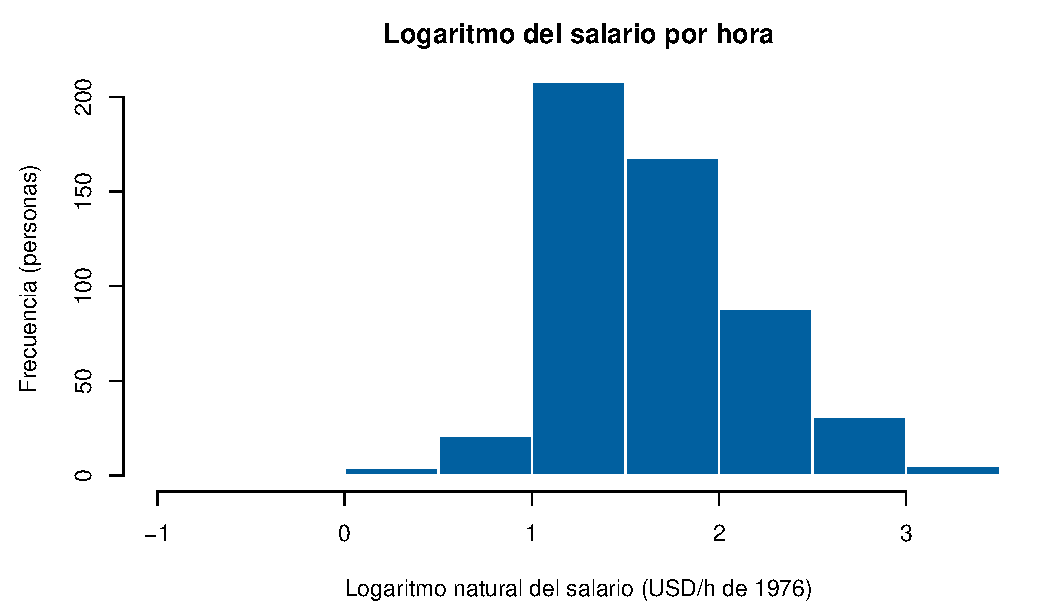
\includegraphics[width=0.96\linewidth]{respuestas-taller-1-figuras/respuesta-5.pdf}\end{center}

\textbf{Descripción de lo observado.} El histograma concentra la mayoría de los valores del logaritmo del salario entre 1 y 2, y presenta una cola hacia valores más altos. Hay pocas observaciones en los extremos. El eje vertical cuenta personas; el horizontal muestra el logaritmo natural del salario por hora, no el salario original.

Un valor negativo en el eje horizontal no significa un salario negativo: significa que el salario original es positivo y menor que 1 USD por hora. La transformación comprime las diferencias entre salarios altos. En esta base, la media salarial original es aproximadamente \textbf{5,896 USD/h} y su mediana es \textbf{4,650 USD/h}; no deben confundirse con los valores de la escala logarítmica.

\textit{Datos: 526 personas de la CPS de Estados Unidos, 1976. Para verificar las respuestas se utilizó la copia local de wage1, sin cambiar sus valores.}
\newpage
\respuesta{6. Salarios según antigüedad}
\begin{lstlisting}
datos$tenure_grupo <- cut(
  datos$tenure, breaks = c(-Inf, 0, 3, 8, Inf),
  labels = c("0", "1 a 3", "4 a 8", "Más de 8"),
  right = TRUE
)
table(datos$tenure_grupo)
boxplot(wage ~ tenure_grupo, data = datos,
        col = c("#0160a0", "#f8c751", "#00875a", "#e12523"),
        main = "Salario según antiguedad con el empleador",
        xlab = "Antigüedad (años)",
        ylab = "Salario por hora (USD de 1976)")
aggregate(wage ~ tenure_grupo, data = datos, FUN = median)
\end{lstlisting}
\begin{center}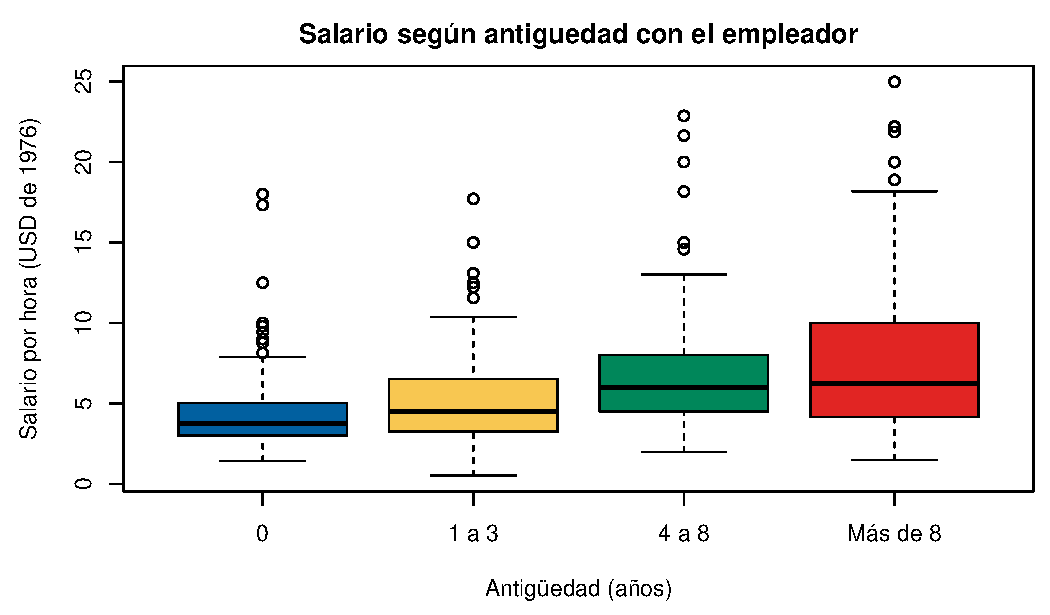
\includegraphics[width=0.96\linewidth]{respuestas-taller-1-figuras/respuesta-6.pdf}\end{center}

\begin{center}
\begin{tabular}{lrrr}
\toprule
\textbf{Antigüedad} & \textbf{Personas} & \textbf{Media (USD/h)} & \textbf{Mediana (USD/h)}\\
\midrule
0 años & 163 & 4,531 & 3,750\\
1 a 3 años & 156 & 5,362 & 4,505\\
4 a 8 años & 102 & 6,908 & 6,000\\
Más de 8 años & 105 & 7,826 & 6,250\\
\bottomrule
\end{tabular}
\end{center}
Las medianas aumentan entre los grupos, aunque las distribuciones se superponen. El grupo de más de 8 años presenta una caja más amplia y se observan valores altos fuera de los bigotes en todos los grupos. Estos puntos no son automáticamente errores. La comparación describe una asociación y no prueba que aumentar la antigüedad cause por sí solo un aumento salarial.

Con \codigo{right = TRUE}, cada intervalo incluye su límite derecho: 0 queda en el primer grupo, 3 en el segundo y 8 en el tercero. Los cuatro grupos reúnen las 526 personas de la base.
\newpage
\respuesta{7. Histograma de promedios muestrales}
\begin{lstlisting}
avg_wage <- numeric(1000)
set.seed(123)
for (i in 1:1000) {
  filas <- sample(1:nrow(datos), size = 50, replace = FALSE)
  avg_wage[i] <- mean(datos$wage[filas])
}
hist(avg_wage, main = "Promedios salariales de 1000 muestras",
     xlab = "Promedio salarial (USD/h de 1976)",
     ylab = "Frecuencia de muestras",
     col = "#0160a0", border = "white")
head(avg_wage)
mean(avg_wage)
sd(avg_wage)
\end{lstlisting}
\begin{center}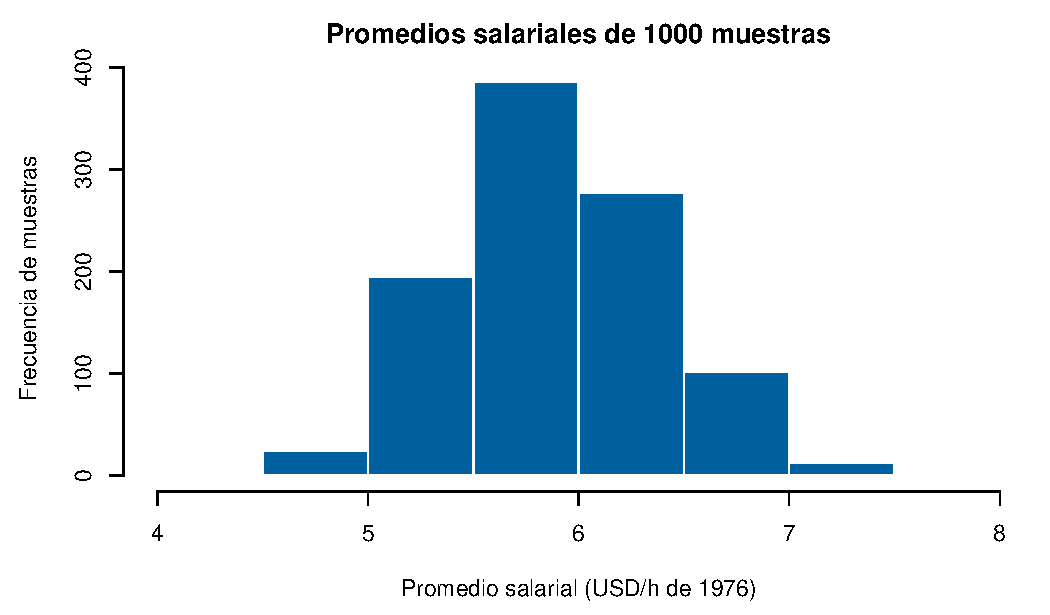
\includegraphics[width=0.96\linewidth]{respuestas-taller-1-figuras/respuesta-7.pdf}\end{center}

\textbf{Descripción de lo observado.} Se observa una distribución unimodal, aproximadamente acampanada, con la mayor concentración de promedios alrededor de 5,9 USD/h y pocos valores en los extremos. La figura muestra la distribución de \textbf{1.000 promedios muestrales}, no la de 1.000 salarios individuales.

\textbf{La forma aproximadamente acampanada de esta distribución es evidencia empírica compatible con el Teorema Central del Límite en este experimento.}

Con \codigo{set.seed(123)}, los primeros seis promedios son \textbf{5,9300; 5,7710; 4,7260; 6,4020; 6,3214 y 5,5564}. La media de los 1.000 promedios es aproximadamente \textbf{5,8964 USD/h} y su desviación estándar es \textbf{0,5006 USD/h}.

La semilla se fija una sola vez, antes del ciclo. Dentro de cada muestra no se repiten filas; entre distintas muestras sí pueden volver a aparecer. \codigo{avg_wage[i]} guarda un promedio por posición.
\newpage
\respuesta{8. Educación, experiencia y correlación}
\begin{lstlisting}
plot(datos$educ, datos$exper, pch = 19,
     col = "#0160a080", main = "Educación y experiencia laboral",
     xlab = "Educación (años)", ylab = "Experiencia (años)")
cor(datos$educ, datos$exper)
\end{lstlisting}
\begin{center}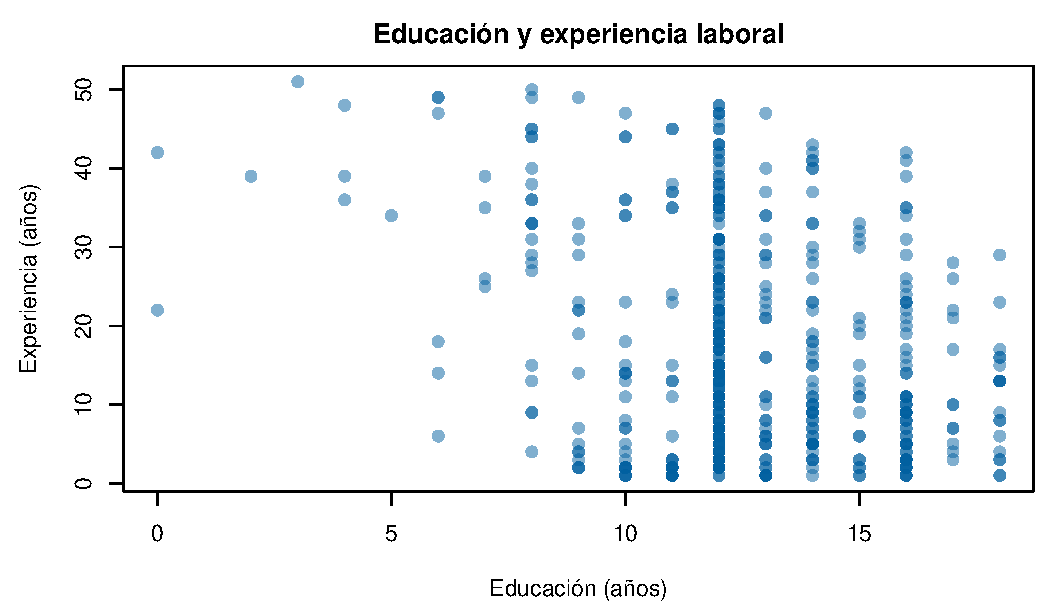
\includegraphics[width=0.96\linewidth]{respuestas-taller-1-figuras/respuesta-8.pdf}\end{center}

La correlación de Pearson es aproximadamente \textbf{$r=-0{,}2995$}. No se observa una relación lineal marcada entre los años de educación y la experiencia laboral. Al comparar los valores cercanos a 0 años de educación con los superiores a 15 años, se aprecia una tendencia negativa. Sin embargo, la experiencia varía mucho dentro de cada nivel educativo, lo que hace que la relación sea débil. El coeficiente se calcula con todas las observaciones, no solo con esos extremos.

Las columnas de puntos se deben a que muchas personas tienen la misma cantidad de años de educación. A un mismo nivel educativo se observan diferentes años de experiencia. El coeficiente no es cercano a $-1$, por lo que la relación no es una línea descendente perfecta.

Esta comparación no demuestra causalidad. La edad y otras características pueden relacionarse con ambas variables; el gráfico y la correlación no las mantienen constantes.

\end{document}
